% Optimal truncation
\section{Optimal Truncation}
\label{sec:truncation}

In any decomposition-based approximation the question emerges of how many terms to keep. The optimal value depends both on the true rank of the underlying signal but also the signal to noise ratio: truncating the decomposition of a rank $r$ data matrix at $r$ does not necessarily give the result that minimizes error. Almost always, the suggestion is to use a heuristic method, but it turns out that one can do better. The discussion below uses the context of singular value decomposition, but the problem of optimal truncation is more general and is an example tuning the hyperparameter that determines the capacity of an estimator to mold itself to a dataset.


\subsection{Scree Plots, Heuristic Methods}
\label{sec:scree}
The canonical heuristic approaches focus on \textit{scree plots}, which simply show the singular values in decreasing order, or cumulative plots, which show the fraction of the total sum of singular values that the first $n$ singular values add up to. In case of PCA, the cumulative plot is directly interpretable as the fraction of the explained variance by the first $n$ principal components, where the total variance is given by $\sigma_2 = \sum_i \sigma_i^2$. \\

A scree plot is sometimes referred to as an \textit{elbow plot}, and a common approach is to truncate at the elbow, which is known as \textit{elbow truncation}. Scree refers to the rock fragments that gather at the foot of a steep hill due to erosion, but I wouldn't really know, because I haven't gone outside in a while. 

Another common way to go about this would be to, for example, keep only the singular components that account to 90\% of the decomposition.

\begin{figure}
\centering
    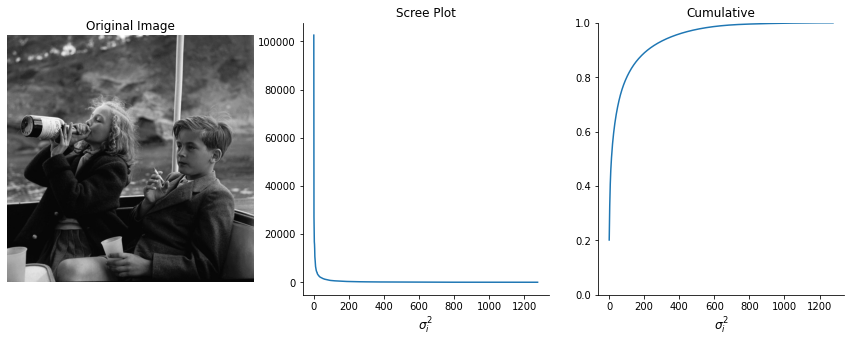
\includegraphics[width=\textwidth]{svd_scree.png}
    \caption{Left: Original image of Princess Yvonne und Prince Alexander zu Sayn-Wittgenstein, photographed by their mother, Princess Marianne, in 1955 (1280 by 1277 pixels). Middle: Scree plot, which shows that the first few components are dominant in the image. Right: Cumulative plot that shows that the first singular component accounts for more than 20\% of the decomposition.}
    \label{fig:svd_scree}
\end{figure}


Either method is not limited to SVD or PCA, but also show up whenever, for example, someone wants to decide on the number of clusters in cluster analysis, the number of regressors in mutlivariate regression (only sometimes), or independent component analysis (ICA).


\subsection{Gavish \& Donoho's Optimal Threshold for SVD}

I came across this through \citeasnoun{gavish2013optimal} and Steve Brunton's youtube channel \cite{stevebrunton}. The idea is the following. Assume that some data matrix $\mathbf{X}\in\mathbb{R}^{N \times p}$ consists of a signal $\mathbf{X}_{r}$ with a rank $r$ substructure, and normally distributed noise with mean zero $\mathbf{X}_{\epsilon}\sim \mathscr{N}(0,\sigma_{\epsilon}^2)$. The method assumes that the rank of the signal $r$ is small compared to the rank of $\mathbf{X}$. 

\begin{equation}
\mathbf{X} = \mathbf{X}_r + \mathbf{X}_{\epsilon}
\end{equation}

The distribution of singular values of a matrix $\mathbf{X}_{\epsilon}\sim \mathscr{N}(0,\sigma_{\epsilon}^2)$ is known up to the variance. \possessivecite{gavish2013optimal} method is to truncate the decomposition of $\mathbf{X}$ at the singular value that fall below the largest singular value of $\mathbf{X}_{\epsilon}$. It turns out that, with respect to average mean square error, this truncation is asymptotically always better than any other truncation and even always better than the true thresholding at rank $r$ when the rank of the underlying signal happens to be known. When the variance of the noise $\sigma^2_{\epsilon}$ is not known, then \citeasnoun{gavish2013optimal} instead use the median singular value of $\mathbf{X}$. 

Let $y_{\mathrm{med}} = \mathrm{med}\{\sigma_i: 1\leq0\leq n\}$ be the median singular value. Then the optimal hard threshold for a matrix $\mathbf{X}\in\mathbb{R}^{m \times n}$ is given by:

\begin{equation}
\tau = \omega(\beta) y_{\mathrm{med}}
\end{equation}

Where $\beta= \frac{m}{n}$ is the aspect ratio of the matrix $\mathbf{X}$ so that $0\leq \beta \leq 1$,  and $\omega(\beta)$ is a constant that needs to be calculated numerically:

\begin{equation}
\omega(\beta) = \frac{\lambda_{*}(\beta)}{\sqrt{\mu_{\beta}}}
\end{equation}

Where $\lambda_{*}(\beta)$:

\begin{equation}
\lambda_{*}(\beta) = \sqrt{2(\beta+1) + \frac{8\beta}{(\beta+1)+\sqrt{\beta^2 + 14\beta+1}}} 
\end{equation}

And $\mu_{\beta}$ is unfortunately the median of the Mar\v{c}enko-Pastur distribution, which is the unique solution to:

\begin{equation}
\int_{\beta_{-}^x}\frac{\sqrt{(\beta_{+}-t)(t-\beta_{-})}}{2\pi t} \mathrm{d}t = \frac{1}{2}
\end{equation}

With $\beta_{\pm} = (1\pm\beta)^2$. Cautiously, \citeasnoun{gavish2013optimal} provide the approximation:

\begin{equation}
\omega(\beta) \approx 0.56\beta^3 - 0.95\beta^2 + 1.82\beta + 1.43
\end{equation}

Which has error bounded by $\leq0.02$ on the interval $0.001\leq\beta \leq 1$.


\begin{figure}
\centering
    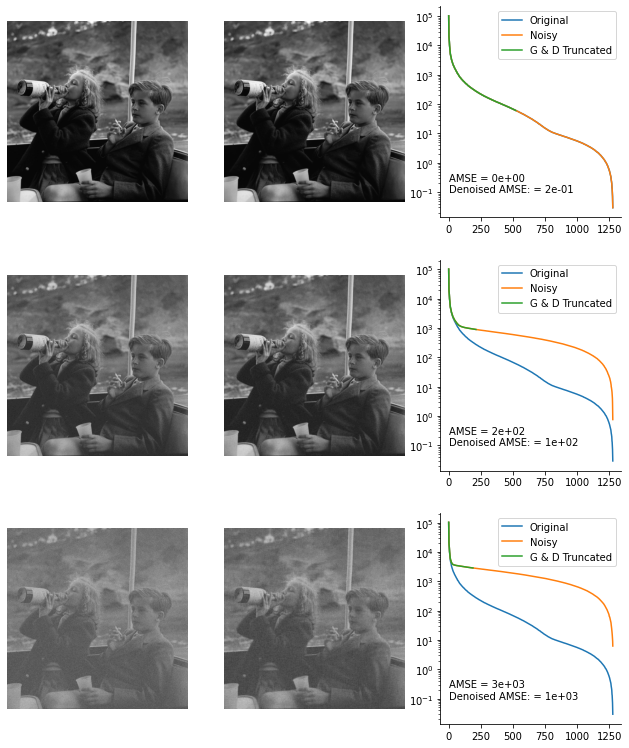
\includegraphics[width=\textwidth]{truncated_svd.png}
    \caption{Left: Princess and Prince zu Sayn-Wittgenstein with different amounts of Gaussian noise added. Center: The same image estimated using TSVD with Gavish \& Donoho's approximate rank threshold. Right: Singular value spectrum of original, noise and truncated images. TSVD reduces the average mean square error (AMSE) with respect to the original image by over 50\%. Visually, the difference is not too perceptible.}
    \label{fig:truncated_svd}
\end{figure}